\chapter{Ocean-atmosphere vertical column modelling}
\label{ch:airseaSCM}
\minitoc
We present in this chapter the concepts and equations at
the continuous level which
will be used in the rest of this thesis.
In particular, in Section \ref{sec:airseaSCM_primitiveEquations}
the primitive equations describing the large-scale
oceanic and atmospheric circulation are derived; then
the turbulent features are described in Section
\ref{sec:airseaSCM_turbulence}.
Finally, the simplified models used in this thesis are summed up
in Section \ref{sec:airseaSCM_hierarchy},
before discussing Schwarz methods in Section
\ref{sec:airseaSCM_Schwarz}.
\section{Derivation of the primitive equations}
\label{sec:airseaSCM_primitiveEquations}
This section aims to present the so-called
primitive equations, which are used to model the fluid dynamics
in the inner parts of both the atmosphere and ocean. They represent
a classical choice for studying climate and weather predictions.
\subsection{Unaveraged primitive equations}
\label{sec:airseaSCM_nonTurbulentPrimitiveEq}
We start from the \textit{Navier-Stokes momentum equation}
in a rotating frame
which describes the evolution of the momentum $\rho \mathbf{U}$
(the symbols are given in Table
\ref{tab:airseaSCM_primitiveEquationsSymbols}):
\begin{equation}
\label{eq:airseaSCM_momentumNavierStokes}
\rho \underbrace{
\left(\partial_t + \mathbf{U} \cdot \nabla \right)
	}_{\text{Material derivative}} \mathbf{U}
=
\underbrace{
	- \nabla p
}_{\text{Pressure gradient}}
+
\underbrace{
	K_{u, {\rm mol}} \Delta \mathbf{U}
}_{\text{Molecular diffusion}}
-
\underbrace{
	\rho \mathbf{g}
}_{\text{Gravity}}
-
\underbrace{
2 \mathbf{\Omega} \times (\rho \mathbf{U})
}_{\text{Coriolis effect}}
\end{equation}
\begin{table}
\centering
\begin{tabular}{c|c|c}
Symbol & Quantity & Unit \\
\hline
$\rho$& {Density} & ${\rm kg}.{\rm m}^{-3}$ \\
$p$   & {Pressure} & ${\rm kg}.{\rm m}^{-1}.{\rm s}^{-2}$ \\
$\mathbf{U}$ & {Velocity}& ${\rm m}.{\rm s}^{-1}$ \\
$\theta$ & {Potential temperature}& ${\rm K}$ \\
$K_{u, {\rm mol}}$ & {Molecular viscosity}& ${\rm m}^{-1}.{\rm s}^{-2}$ \\
$\mathbf{g}$ & {Gravity acceleration}& ${\rm m}.{\rm s}^{-2}$ \\
$\mathbf{\Omega}$ & {Earth angular speed}& ${\rm rad}.{\rm s}^{-1}$ \\
$\nabla$ & {Spatial Gradient} & ${\rm m}^{-1}$\\
$\Delta$ & {Spatial Laplacian} &${\rm m}^{-2}$
\end{tabular}
\caption{Symbols used in Section
\ref{sec:airseaSCM_primitiveEquations}. Bold letters
indicate that the quantity lies in $\mathbb{R}^3$.}
\label{tab:airseaSCM_primitiveEquationsSymbols}
\end{table}
and the \textit{continuity equation} which ensures
conservation of mass:
\begin{equation}
\label{eq:airseaSCM_conservationMass}
\partial_t \rho = - \nabla \cdot (\rho \mathbf{U})
\end{equation}
In the three components of
$\mathbf{U} = \begin{pmatrix}u\\v\\w\end{pmatrix}$, $u$ and $v$
correspond to the horizontal velocities (in $x$ and $y$ directions)
and $w$ is the vertical velocity (the vertical axis is noted
with the letter $z$).
Some common approximations simplify the two equations
\eqref{eq:airseaSCM_momentumNavierStokes} and
\eqref{eq:airseaSCM_conservationMass}:
\begin{itemize}
\item \textit{Spherical geoid approximation}:
we assume that the earth is spherical and that the
gravity acceleration is given by
$\mathbf{g} =\begin{pmatrix}
	\emphase{0}\\ \emphase{0} \\ g
\end{pmatrix}$ where $g\approx 9.81 {\rm m}.{\rm s}^{-2}$.
\item \textit{Traditional approximation}:
We neglect the horizontal terms of
the rotation vector $\mathbf{\Omega}$
involved in the Coriolis force: we assume that
$\mathbf{\Omega} =\begin{pmatrix}
	\emphase{0}\\ \emphase{0} \\ f/2
\end{pmatrix}$ where $f$ depends on the latitude.
$f$ is commonly referred to as the Coriolis frequency.
\item \textit{Hydrostatic fluid}:
the vertical pressure gradient balances the gravity force:
$\partial_z p = -\rho g$. The vertical
acceleration is neglected compared to pressure and gravity.
This approximation is usually done in large-scale simulations
when the horizontal
space step is larger than the vertical one by several orders
of magnitude; it is typically the case in climate simulations.
\item \textit{Boussinesq approximation}
\citep{boussinesq_theorie_1903}:
the density $\rho$ is close to a constant $\rho_0$.
The variation of density $\widetilde{\rho} =
\rho - \rho_0$ is neglected except when it is multiplied by $g$
computing in the pressure gradient $\partial_z p = - \rho g$.
The atmosphere models rely on compressibility and
do not use this approximation. However, we make
the Boussinesq approximation for both domains
as we assume that the compressibility effects
are small close to the surface and that they
can be neglected to study the surface layer.
\end{itemize}
We hence obtain the \textit{unaveraged}
primitive equations:
\begin{equation}
	\label{eq:airseaSCM_nonTurbulentPrimitiveEq}
\begin{cases}
	\nabla \cdot \mathbf{U} &= 0 \\
	\partial_t u + \nabla \cdot (\mathbf{U} u) &=
	- \displaystyle \frac{\partial_x p}{\rho_0} + K_{u, {\rm mol}} \Delta u
	+ f v \\
	\partial_t v + \nabla \cdot (\mathbf{U} v) &=
	- \displaystyle\frac{\partial_y p}{\rho_0} + K_{u, {\rm mol}} \Delta v
	- f u \\
	\partial_z p &= -\rho g
\end{cases}
\end{equation}
where the vertical component of the velocity $w$ is implicitly
represented and can be obtained from
$\nabla \cdot \mathbf{U} = 0$.
\paragraph{Stratification}
$\rho$ is given by an equation of state, which only involves
the temperature in our case (in particular, the effect
of humidity (in the atmosphere) and salinity (in the ocean)
are neglected here).
A \textit{neutral} stratification refers to a constant 
density along the vertical axis. Our focus will eventually
be reduced to the vertical axis and we assume for this
reason that the density is a constant along all directions.
A consequence of the density being constant is that
the temperature does not need to be computed
to determine the velocity $\mathbf{U}$.
\par
On the contrary, in a \textit{stratified} case the
density depends on the potential temperature $\theta$
through an equation of state:
\begin{equation}
	\rho = \rho_{\rm eos}(\emphase{\theta})
\end{equation}
and $\theta$ is given by a transport-diffusion equation:
\begin{equation}
	\emphase{\partial_t \theta} +
	\nabla \cdot (\mathbf{U} \emphase{\theta}) =
	K_{\theta, {\rm mol}} \Delta \emphase{\theta} + F_\theta
\end{equation}
where $K_{\theta, {\rm mol}}$ and $F_\theta$ are
the molecular diffusivity and some forcing term.
$\theta$ must be computed jointly with $\mathbf{U}$
to solve the system \eqref{eq:airseaSCM_nonTurbulentPrimitiveEq}.
The coupling between $\theta$ and $\mathbf{U}$ is done through
the pressure gradient.
%
\subsection{Reynolds decomposition}
The solution of the system \eqref{eq:airseaSCM_nonTurbulentPrimitiveEq}
contains very small scales which cannot be solved numerically for
large domains such as the ocean or the atmosphere. It is hence usual
to use the \textit{Reynolds decomposition}, which consists in
separating the variables into an ``average" part which can be
represented by the numerical schemes and a \textit{turbulent}
part which will be parameterized with appropriate turbulence closure
schemes
(detailed later in \S \ref{sec:airseaSCM_turbulentClosure}).
\par
For $X=u, v, w$ or $\theta$, we note
\begin{equation}
	X =
	\underbrace{\langle X\rangle}_{\text{average part}}
	+
	\underbrace{
	\left.X'\right.
}_{\text{turbulent part}}
\end{equation}
where $\langle \cdot \rangle$ represents a \textit{statistical}
average which satisfies:
\begin{equation}
\begin{aligned}
	\langle X' \rangle &= 0 \\
	\langle \partial_\beta X \rangle &=
	\partial_\beta \langle  X \rangle, ~~~\beta=x,y,z,t \\
	\langle\langle \cdot \rangle\rangle &= \langle \cdot \rangle \\
	\langle \langle X \rangle Y\rangle &= \langle X \rangle\langle Y \rangle
\end{aligned}
\end{equation}
Using those properties, the Reynolds decomposition of 
\eqref{eq:airseaSCM_nonTurbulentPrimitiveEq} gives a system
of equations satisfied by the Reynolds-averaged quantities:
\begin{equation}
	\label{eq:airseaSCM_TurbulentPrimitiveEq}
\begin{cases}
	\nabla \cdot \langle\mathbf{U}\rangle &= 0 \\
	\partial_t \langle u \rangle+ \nabla \cdot
	(\langle\mathbf{U}\rangle \langle u\rangle) &=
	- \frac{\partial_x  p}{\rho_0} +
	K_{u, {\rm mol}} \Delta \langle u\rangle
	+ f \langle v\rangle - \emphase{\nabla \cdot \langle
	\mathbf{U}' u'\rangle}\\
	\partial_t \langle v\rangle + \nabla \cdot
	(\langle \mathbf{U}\rangle \langle v\rangle) &=
	- \frac{\partial_y  p}{\rho_0} +
	K_{u, {\rm mol}} \Delta \langle v\rangle
	- f \langle u\rangle  - \emphase{\nabla \cdot \langle
	\mathbf{U}' v'\rangle}\\
	\partial_z p &= -\rho g \\
	\partial_t \langle\theta\rangle + \nabla \cdot
	(\langle\mathbf{U}\rangle \langle\theta\rangle) &=
	K_{\theta, {\rm mol}} \Delta \langle\theta\rangle
	+ F_\theta - \emphase{\nabla \cdot \langle
	\mathbf{U}' \theta'\rangle}\\
	\rho &= \rho_{\rm eos}(\langle\theta\rangle)
\end{cases}
\end{equation}
From now on, this thesis will only focus the vertical terms
$\langle w' u'\rangle$, $\langle w' v'\rangle$ and
$\langle w' \theta'\rangle$
because the surface layer turbulent features are mainly limited
to those terms. For the same reason, we restrict our spatial
domain to one dimension: the equations model a vertical column
of atmosphere and of ocean. Those are common simplifications to
study vertical turbulent mixing problems.
%\par
%The vertical velocity $w$ can be eventually recovered with the
%equation $\nabla \cdot \langle\mathbf{U}\rangle = 0$
%but we will not directly simulate it and examine only
%$\langle u \rangle, \langle v \rangle$ and $\langle \theta \rangle$.
% The prognostic (i.e. explicitly simulated) variables
% are $\langle u \rangle, \langle v \rangle$ and
% $\langle \theta \rangle$.
Finally, note that \eqref{eq:airseaSCM_TurbulentPrimitiveEq}
shoult be completed with initial and boundary conditions:
they will be given for our models of interest in
\S\ref{sec:airseaSCM_WallLaw}.
\par
The non-linear advective terms and the horizontal
pressure gradient term absent from the one dimensional model
will be taken into account through an external \textit{geostrophic}
forcing. The latter represents the geostrophic equilibrium which
is a state of the fluid in which the pressure gradient compensates
the Coriolis effect. This geostrophic forcing reduces
drastically the complexity of the system and keeps
reasonable values
for the variables.
\par
The one-dimensional system of
equations is the following:
\begin{equation}
	\label{eq:airseaSCM_TurbulentPrimitiveEq1D}
\begin{cases}
	\partial_t \langle u \rangle
	+ \emphase{\partial_z \langle w' u'\rangle}
	&=
	K_{u, {\rm mol}} \partial_z^2 \langle u\rangle
	+ f \left(\langle v\rangle - v_G\right)
	\\
	\partial_t \langle v\rangle
	+ \emphase{\partial_z \langle w' v'\rangle}
	&=
	K_{u, {\rm mol}} \partial_z^2 \langle v\rangle
	- f \left(\langle u\rangle-u_G\right)\\
	\partial_t \langle\theta\rangle
	+ \emphase{\partial_z \langle w' \theta'\rangle}&=
	K_{\theta, {\rm mol}} \partial_z^2 \langle\theta\rangle
	+ F_\theta\\
	\rho &= \rho_{\rm eos}(\langle\theta\rangle)
\end{cases}
\end{equation}
where $u_G, v_G$ are the geostrophic velocity.
\par
With this decomposition we obtain more unknown than
equations because of the introduction of the terms
$\langle w' u'\rangle, \langle w' v'\rangle$
and $\langle w' \theta'\rangle$:
this is known as the turbulence closure problem.
The quantities of interest are the averaged quantities
$\langle u\rangle, \langle v\rangle, \langle \theta \rangle$:
a \textit{turbulence closure} defines a relation between
the turbulent terms $\langle w' u'\rangle, \langle w' v'\rangle,
\langle w' \theta'\rangle$ and those averaged quantities.
The density $\rho$ is not used explicitly
in \ref{eq:airseaSCM_TurbulentPrimitiveEq1D}
but appear in the turbulence closure.
\section{The turbulence}
\label{sec:airseaSCM_turbulence}
To tackle the turbulence closure problem,
we now provide additional relations between
the turbulent terms and the average quantities.
We first detail a common choice of parameterization
for the turbulence closure far from the surface and then
(in \S\ref{sec:airseaSCM_WallLaw}) focus on the surface layer
which acts as a bottom boundary condition for
\eqref{eq:airseaSCM_TurbulentPrimitiveEq1D} in the atmosphere.
The ocean case is discussed in \S\ref{sec:airseaSCM_twoSided}.
\subsection{Turbulent closure and kinetic energy}
\label{sec:airseaSCM_turbulentClosure}
\paragraph{Boussinesq hypothesis}
From the observation that the turbulent term acts like a diffusion
term oriented ``down-gradient", the turbulent terms are approximated
with the help of a ``turbulent viscosity" $K_u$ and a
``turbulent diffusivity" $K_\theta$:
\begin{equation}
\emphase{\langle w' u'\rangle =
	- K_u \partial_z \langle u \rangle}, ~~~
\langle w' v'\rangle = - K_u \partial_z \langle v \rangle, ~~~
\langle w' \theta'\rangle =
	- K_\theta \partial_z \langle \theta \rangle
\end{equation}
This is known as the \textit{Boussinesq hypothesis}
(\citep{boussinesq_theorie_1897},
different from the Boussinesq \textit{approximation} neglecting
effects of compressibility)
\par
The turbulent viscosity and diffusivity can be defined in a lot of
different ways. A typical formulation for $K_u, K_\theta$ is
\begin{equation}
	\emphase{K_u} = C_m l_m \emphase{\sqrt{e}}, ~~~~~~~ K_\theta = \frac{C_m}{\rm Pr}
	l_m \sqrt{e}
	= \frac{K_u}{\rm Pr}
\end{equation}
where $C_m$ is a constant; the turbulent Prandtl number
${\rm Pr}$ indicates the ratio of the viscosity to the diffusivity;
the mixing length $l_m$ is a characteristic
length of the turbulent flow and depends on the stratification.
$e$ is an important quantity often used in the turbulence models,
the Turbulent Kinetic Energy (TKE):
\begin{equation}
	e = \frac{1}{2} \left(\langle (u')^2 \rangle + \langle (v')^2 \rangle
	+ \langle (w')^2 \rangle\right)
\end{equation}
The evolution equation for the TKE is
\begin{equation}
	\partial_t e ~~-
\underbrace{\partial_z \left(K_e
    \partial_z e\right)}_{\text{diffusion with } K_e \propto K_u}
    =
	~~\underbrace{P}_{\parbox{25pt}{\scriptsize{ source\\(shear)}}}
	~~~+~~~
	\underbrace{B}_{\parbox{35pt}{\scriptsize{ source/sink\\(buoyancy)}}}
	~~~-~~~
	\underbrace{\epsilon}_{\text{dissipation rate}}
\end{equation}
where $P>0$ and $B$ are terms denoting respectively
the shear and buoyancy production of kinetic energy;
$\epsilon>0$ is the dissipation rate of TKE
into heat.
\par
$P$ corresponds to the energy lost by $\langle u \rangle$ through the
\textit{shear} term
$\partial_z \left(K_u \partial_z \langle u \rangle\right)$:
to compute it, we multiply by $\langle u \rangle$ the equation
$\partial_t \langle u \rangle = \partial_z (K_u \partial_z \langle u \rangle)$
and express the result as a function of the
energy of the mean velocity $\displaystyle\langle u \rangle^2/2$.
This gives (e.g. \citep{burchard_energy-conserving_2002},
where the derivation is done both at the continuous and at the
discrete level):
\begin{equation}
	\partial_t \left(\frac{\langle u \rangle^2}{2}\right)
	- \partial_z \left(K_u
	\partial_z\left(\frac{\langle u \rangle^2}{2}\right)\right)
	= - \emphase{K_u\left(\partial_z \langle u \rangle\right)^2}
\end{equation}
where we deduce that
$P=\emphase{K_u \left(\left(\partial_z \langle u \rangle\right)^2 +
\left(\partial_z \langle v \rangle\right)^2\right)}$ is the energy
\textit{produced} by the shear.
\par
A similar treatment with the density
(whose diffusion term is multiplied by $z$ instead of $\langle u \rangle$)
gives that the potential energy
is increased or reduced by $B = -K_\theta N^2$ where
$N^2 = - \displaystyle {g\partial_z \rho}/{\rho_0}$ is the Brunt-Väisälä
frequency.
The dissipation rate $\epsilon$ can be parameterized by
$\epsilon \propto \displaystyle \frac{e^{3/2}}{l_{\epsilon}(z)}$
where $l_\epsilon$ is a mixing length similar to $l_m$.
This parameterization of $\epsilon$ gives the widely used
\textit{Prandtl's one-equation turbulence model}.
\par
Finally, the one-dimensional evolution equation for the TKE is
\begin{equation}
\label{eq:airseaSCM_TKE_evolution}
    \begin{aligned}
    \partial_t e =
    \underbrace{\partial_z \left(K_e
    \partial_z e\right)}_{\text{diffusion}}
	    + \underbrace{K_u \left(\left(\partial_z
	    \langle u \rangle\right)^2 +
	    \left(\partial_z \langle v \rangle\right)^2\right)
	    }_{\parbox{25pt}{\scriptsize{ source\\(shear)}}}
    ~~-~~ \underbrace{K_{\theta} N^2
    }_{\parbox{35pt}{\scriptsize{ source/sink\\(buoyancy)}}}
    ~~-~~ \underbrace{c_{\epsilon}
    \frac{e^{3/2}}{l_{\epsilon}(z)}}_{\text{dissipation}}
    \end{aligned}
\end{equation}
The equation \eqref{eq:airseaSCM_TKE_evolution} is used as a model
of the turbulent energy: $e$ is jointly integrated in time with
$\langle \mathbf{U} \rangle, \langle \theta \rangle$
and is used to characterize the turbulent terms appearing
in \eqref{eq:airseaSCM_TurbulentPrimitiveEq1D}.
From now on, the operator $\langle \cdot \rangle$ will be omitted
and the letters $u, v, \theta$ will refer to the averaged variables
$\langle u \rangle, \langle v \rangle, \langle \theta \rangle$.
\par
This model is only accurate outside the surface layer. The latter
offers boundary conditions for the turbulent terms and is discussed
in the next \S.
\subsection{Law of the wall and Monin-Obukhov Similarity Theory}
\label{sec:airseaSCM_WallLaw}
% Pour l'hypothèse de surface libre: c'est en fait une conséquence de négliger l'humitidé. L'océan ne change pas de volume C'est une hypothèse qui est faite en pratique de considérer l'océan comme ayant une géométrie plane.  Même ayant une surface libre dans l'océan, l'atmosphère le voit comme une surface plane Mais en 1D la question se pose pas.  Du coup on peut ptet l'enlever du chap1 In all this thesis, we will assume that the water surface is flat: this restriction strongly simplifies
% the column models, in particular when the space step becomes
% smaller than the surface waves.
% The free ocean surface is beyond the scope of this thesis:
% however, excluding explicitly
% the surface layer from the computational
% domain (like it will be done in Chapters \ref{ch:ND},
% \ref{ch:OceanND}) may lead to
% a relatively simple handling of the free surface.
We call \textit{surface layer} the area close to the ocean surface
such that it responds to a change at the surface with a ``short"
timescale\footnote{In the literature, a boundary layer can also
be defined as the region in which the fluid goes from zero
velocity to the maximum velocity: this definition is however
less adapted to the oceanic surface layer where the currents
are driven by the surface wind.}.
Wall modelling gives us a description of the surface layer
and provides the boundary conditions for
$\langle w' u'\rangle, \langle w' v'\rangle$ and
$\langle w' \theta'\rangle$.
\par
One of the main hypothesis of the wall modelling is that
the interface is a rough surface.
Indeed, for the atmosphere the ocean surface can be seen as
rough: the wind cannot slip on the ocean which
means that the velocity of the wind is zero relatively
to the surface.
% \par
% \myTD{copié-collé du chapitre 4:}
% \par
% In fluid dynamics, the presence of a rough surface makes strong
% gradients appear:
% due to the no-slip boundary condition
% the scales of motion close to the surface are much smaller than
% elsewhere in the domain and it is numerically
% intractable in most applications
% to refine the mesh enough for those small scales.
% The models hence exclude from the computational domain
% a part of the surface layer, using an adapted boundary
% condition.
%
\paragraph{Neutral case}
We first present the case without stratification:
\citep{karman_mechanische_1930} noticed that the
fluids close to rough surfaces present similarities and
proposed a universal function based on dimensional analysis.
Von K\'arm\'an also states that ``the characteristic length
of the flow pattern is proportional to
[the distance to the wall]".
\par
\begin{figure}[h!]
	\centering
	\subimport{images/}{EddiesDrawing.pdf_tex}
	\caption{The characteristic size of the eddies
	(in purple) is proportional to the distance to the
	surface. The link between the size of the eddies
	and the logarithmic profile (in orange) is
	the constant flux approximation.
	}
	\label{fig:airseaSCM_eddiesDrawing}
\end{figure}
We list below the main features of the surface layer:
\begin{itemize}
	\item the Coriolis effect and the geostrophic forcing are
		neglected (we assume that the effect of the
		proximity to the surface is predominant);
	\item it is well mixed: the governing equation
		is quasi-stationary (the surface layer
		immediately adjusts to the external parameters).
		As a consequence, the fluxes
		$\langle w'u'\rangle = -K_u \partial_z u$
		and
		$\langle w'v'\rangle = -K_u \partial_z v$
		are constant along the vertical axis.
	\item The vertical profile of $K$ strongly depends 
		on $z$.
		The size of the turbulent eddies at height $z$
		is proportional to the distance to the surface $z$
		(e.g. \citep{kawai_wall-modeling_2012}, see Figure
		\ref{fig:airseaSCM_eddiesDrawing}).
		As a consequence, the turbulent viscosity
		linearly scales with $z+z_u$:
		\begin{equation}
			K_u \propto z+z_u
		\end{equation}
		where $z_u$ (detailed later) accounts for both the
		molecular viscosity and the geometry of the surface.
		In the stratified case we also have for the turbulent
		diffusivity $K_\theta \propto z+z_\theta$.
\end{itemize}
We first assume that it is aligned with the
direction of $u$: since the Coriolis effect
is neglected and the turbulence is assumed isotropic,
there is no rotation of the fluid inside the surface layer
and we can assume without loss of generality that $v=0$
(with a possible rotation of the axes).
We will use the orientation of the wind speed later.
\par
Let us define the \textit{friction scale} $u_\star$
such that\footnote{If $v\neq 0$ then
the formula reads instead $u_\star^2=\sqrt{\langle w' {u'} \rangle^2
+\langle w' {v'} \rangle^2 }$.}
$u_\star^2 = |\langle w' {u'} \rangle|$ and
we have that $z_{u} = z_{u}(K_{\rm mol}, u_\star)$
(see e.g. \citep{schlichting_boundary_1960}
for the choice of $z_{u}$ as a constant
of integration).
\par
Finally, the profiles of $u$ can be integrated vertically with
the two equations
\begin{equation}
	K_u\partial_z u=u_\star^2 ~~~~~~~
	K_u= \kappa u_\star (z+z_u)
\end{equation}
and we obtain the law of the wall which reads:
\begin{equation}
	\label{eq:airseaSCM_LawOfWallProfile}
	\emphase{u(z)} - u(0) = \frac{u_\star}{\kappa}
	\emphase{\ln}\left(\frac{z+z_u}{z_u}\right)
	~~~~~ \forall z\in [0,\delta_{\rm a}]
\end{equation}
where $\kappa = 0.4$ is the Von K\'arm\'an constant. 
$\delta_{\rm a} \approx 10\;{\rm m}$ is the height of
the atmospheric surface layer.
\begin{remark}
	Generally, the law of the wall
	refers to an expression using
	$\ln(\frac{z}{z_u})$. By using $z+z_u$
	instead of $z$,
	the molecular sub-layer is included
	inside the law of the wall: we can hence
	use the profile of $u$ for small $z$
	\citep{pelletier_two-sided_2021}.
	This formulation is not standard but it is
	appropriate for mathematical analyses and
	it does not change the results
	significantly.
\end{remark}
\paragraph{Stratified case}
The extension of the law of the wall to stratified
fluids is called \textit{Monin-Obukhov Similarity Theory}.
It is used in all ocean-atmosphere coupled methods to our knowledge.
The quasi-stationarity is also assumed for the temperature
and $K_u \partial_z u$ and $K_\theta \partial_z \theta$
are both constant along the vertical axis.
We can define a friction scale $\theta_\star$
for the potential temperature, such that
\begin{equation}
	\langle w' \theta' \rangle = u_\star \theta_\star
\end{equation}
\begin{figure}[h!]
	\centering
	\subimport{images/}{turbulent_term.pdf_tex}
	\caption{Summary of the turbulent term handling}
	\label{fig:airseaSCM_turbulentTermHandling}
\end{figure}
Figure \ref{fig:airseaSCM_turbulentTermHandling} summarizes the
handling of the turbulent terms in the stratified case.
To describe the stratification, the \textit{Obukhov length}
is used:
\begin{equation}
	L_{MO} = \frac{u_\star^2}{g \kappa
	\frac{\theta_\star}{\theta(\delta_{\rm a})}}
\end{equation}
which is the only characteristic length describing
accurately the effect of the stratification in
the surface layer \citep{obukhov_turbulence_1946}.
$L_{MO}>0$ in stable stratifications
(where $\theta_\star>0$)
and $L_{MO}<0$ in unstable stratifications
(where $\theta_\star>0$).
The neutral case will be recovered
for $L_{MO} \rightarrow \infty$, corresponding
to $\theta_\star \rightarrow 0$.
\par
Note that the potential temperature at the very top of the surface
layer $\theta(\delta_{\rm a})$ is used. Indeed, the surface layer is
usually driven by the values of $u, \theta$
computed at $\delta_{\rm a}$.
\par
The difference with the neutral case is then contained
in \text{stability functions} $\phi_m, \phi_h$:
\begin{equation}
\begin{aligned}
	K_u &\propto (z+z_u)~
	\emphase{\phi_m\left(\frac{z}{L_{MO}}\right)} \\
	K_\theta &\propto (z+z_u)~
	\emphase{\phi_h\left(\frac{z}{L_{MO}}\right)}
\end{aligned}
\end{equation}
Typical stability functions are plotted in the left panel of Figure
\ref{fig:airseaSCM_stabilityfunctions}.
\begin{figure}[h!]
	\centering
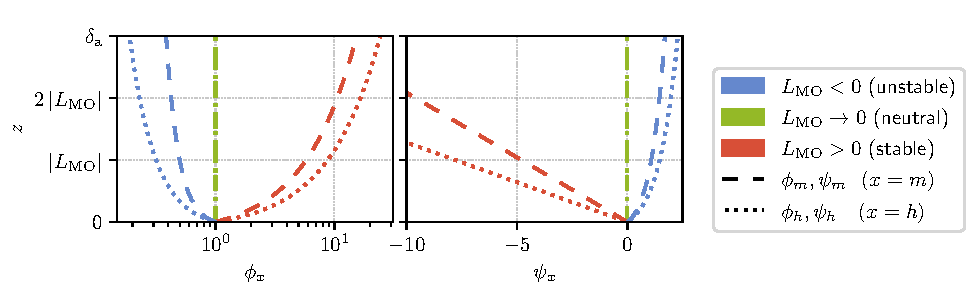
\includegraphics[scale=0.8]{images/stabilityfunctions.pdf}
	\caption{Typical profiles of the stability functions (left)
	and of their integrated form (right) in the
	surface layer $[0,\delta_{\rm a}]$. In the unstable
	and stable cases, $\frac{\delta_{\rm a}}{L_{\rm MO}}$
	was arbitrarily set to respectively -3 and 3.
	}
	\label{fig:airseaSCM_stabilityfunctions}
\end{figure}
A stable (resp. unstable) stratification leads to a
decrease (resp. increase) of $K_u, K_\theta$ and
$L_{MO}\rightarrow \infty$ indeed recovers the neutral case.
To obtain the solution profiles,
the \textit{integrated forms}
of the stability functions $\psi_m, \psi_h$
are defined as
\begin{equation}
	\emphase{\psi_x}\left(\frac{z}{L_{MO}}\right)
	= \emphase{\int_0^{\frac{z}{L_{MO}}}}
	\frac{1 - \emphase{\phi_x}(\zeta)}{\zeta} d\zeta
	, ~~~~x=m,h
\end{equation}
and we have
\begin{equation}
\label{eq:airseaSCM_MOSTprofiles}
\begin{aligned}
	u(z)-u(0) = \frac{u_\star}{\kappa}
    \left(
	\ln(1+\frac{z}{z_{u}})
	\emphase{- \psi_m\left(\frac{z}{L_{MO}}\right)}
    \right)
    \\
    \theta(z) - \theta_s = 
	\frac{\emphase{\theta_\star}}{\kappa}
    \left(
	\ln(1+\frac{z}{z_{\theta}})
	\emphase{- \psi_h\left(\frac{z}{L_{MO}}\right)}
\right)
\end{aligned}
\end{equation}
where $\theta_s$ is the surface temperature.
Monin-Obukhov Similarity Theory
is extensively used (e.g. \citep{basu_cautionary_2017});
it is however not universally
accepted in particular in very stable stratifications
(see \citep{optis_moving_2014}).
\paragraph{Bulk algorithm}
Using \eqref{eq:airseaSCM_MOSTprofiles} and the values of
$u(\delta_{\rm a}) - u(0)$ and $\theta(\delta_{\rm a}) - \theta_s$
it is possible to compute the friction scales
$u_\star, \theta_\star$. It is however not trivial as
$L_{MO}$ and $z_u, z_\theta$ depend themselves on
$u_\star, \theta_\star$.
The so-called ``bulk algorithms" are designed for this
task: they generally rely on a fixed-point method:
\begin{enumerate}
\item input: $u(\delta_{\rm a}) - u(0)$
		and $\theta(\delta_{\rm a}) - \theta_s$;
\item choose a first guess $u_\star^{n=0}, \theta_\star^{n=0}$;
\item iteratively apply
	\eqref{eq:airseaSCM_MOSTprofiles} (or
	\eqref{eq:airseaSCM_LawOfWallProfile} in the neutral case)
	to compute $u_\star^{n}, \theta_\star^{n}$ using
	$u_\star^{n-1}, \theta_\star^{n-1}$
	in the expressions of $z_u, z_\theta$ and $L_{MO}$;
\item at convergence i.e. ($u_\star^{n},\theta_\star^{n}) \approx
	(u_\star^{n-1},\theta_\star^{n-1}$), return the friction
		scales $u_\star = u_\star^{n},
		\theta_\star = \theta_\star^{n}$ (or only
		$u_\star = u_\star^{n}$ in the neutral case)
\end{enumerate}
The bulk formulation is generally part of the atmosphere models and
is essential to compute the surface boundary conditions given the
typical grid resolution in numerical models.
The convergence of this fixed point method 
is discussed in \citep{thery_etude_2021}.
\subsection{Two-sided bulk}
\label{sec:airseaSCM_twoSided}
The ocean and atmosphere have not been distinguished in equations
so far. From this point, we will use a subscript ``o" for the ocean
quantities and ``a" for the atmosphere quantities.
In Chapter \ref{ch:OceanND} we will also consider the
\textit{oceanic surface layer}.
In actual numerical models the sea surface temperature and the
surface currents are often
evaluated taking values below the surface. The common approach is
to neglect the difference between the temperature and currents
at the surface and typically one meter below. However,
\citep{donlon_toward_2002} show that
the difference between
the surface temperature and the sub-surface temperature is
approximatively constant for medium and strong winds but that 
it is harder to evaluate in stratified condition corresponding
to winds slower than $6 \; {\rm m}.{\rm s}^{-1}$).
\citep{ward_near-surface_2006}
``\textit{show the strong dependency of the SST on air-sea heat
flux estimates, with warm-layer errors of almost
60 ${\rm W}.{\rm m}^{-2}$ associated with intense stratification. This indicates
the importance of the inclusion of the skin temperature for
accurate calculation of latent, sensible, and net longwave
heat fluxes}".
In \citep{pelletier_two-sided_2021} a non-standard bulk formulation
which uses Monin-Obukhov Similarity Theory (MOST) in the oceanic
surface layer is derived.
\begin{figure}[h!]
	\centering
	\subimport{images/}{drawingPelletierTwoSided.pdf_tex}
	\caption{Comparison between one-sided (left) and two-sided
	(right) bulk formulations. The gradient discontinuity at zero
	comes from the difference in density.
	Adapted from \citep{pelletier_two-sided_2021}.
	}
	\label{fig:airseaSCM_OSTSBulk_drawing}
\end{figure}
Figure \ref{fig:airseaSCM_OSTSBulk_drawing} shows the difference
between the one-sided and the two-sided bulk formulations.
We follow this idea and incorporate to our coupled model an
oceanic surface layer which follows the same principles as
the surface layer in the atmosphere.
\par
The application of MOST will yield the ocean counterpart
of \eqref{eq:airseaSCM_MOSTprofiles} with different
friction scales. The continuity of the fluxes across the interface
\begin{equation}
	\left.\rho_{\rm a} K_{u,{\rm a}}
	\partial_z u_{\rm a}\right|_{z=0} = 
	\left.\rho_{\rm o} K_{u,{\rm o}}
	\partial_z u_{\rm o}\right|_{z=0}, ~~~~~~
	\left.\rho_{\rm a} K_{u,{\rm a}}
	\partial_z \theta_{\rm a}\right|_{z=0} = 
	\left.\rho_{\rm o} K_{u,{\rm o}}
	\partial_z \theta_{\rm o}\right|_{z=0}
\end{equation}
adds the constraint that the friction scales of the ocean are
$\sqrt{\frac{\rho_{\rm a}} {\rho_{\rm o}}} u_\star$ and
$\sqrt{\frac{\rho_{\rm a}}{\rho_{\rm o}}
\frac{c_{\rm a}^p}{c_{\rm o}^p}}
\theta_\star$ where $c_{\rm o}^p, c_{\rm a}^p$
are the heat capacities of water and air.
We hence have for $\delta_o \leq z \leq 0$ (where $\delta_o \leq 0$
is the depth of the surface layer):
\begin{equation}
	\begin{aligned}
	|K_u \partial_z u_{\rm o}| &= \emphase{\frac{\rho_a}{\rho_o}}
	u_\star^2\\
	K_\theta \partial_z \theta_{\rm o} &=
	\emphase{\frac{\rho_{\rm a} c_{\rm a}^p}
			{\rho_{\rm o} c_{\rm o}^p}}
	\theta_\star u_\star
	\end{aligned}
\end{equation}
and the reconstruction of $u_{\rm o}$, $\theta_{\rm o}$
follow equations similar to \eqref{eq:airseaSCM_MOSTprofiles}:
\begin{equation}
\label{eq:airseaSCM_MOSTprofilesOSL}
\begin{aligned}
	u_{\rm o}(0)-u_{\rm o}(z) = \emphase{\frac{\rho_a}{\rho_o}}
	\frac{u_\star}{\kappa}
    \left(
	\ln(1-\frac{z}{z_{u}^o})
	\emphase{- \psi_m^o\left(-\frac{z}{L_{MO}}\right)}
    \right)
    \\
	\theta_s - \theta_{\rm o}(z) = 
	\emphase{\sqrt{\frac{\rho_{\rm a}}{\rho_{\rm o}}
	\frac{c_{\rm a}^p}{c_{\rm o}^p}}}
	\frac{{\theta_\star}}{\kappa}
    \left(
	\ln(1-\frac{z}{z_{\theta}^o})
	\emphase{- \psi_h^o\left(-\frac{z}{L_{MO}}\right)}
\right)
\end{aligned}
\end{equation}
If $\delta_o$ is set to zero, then there is no surface layer
in the ocean and we call the surface layer \textit{one-sided}.
In the other case ($\delta_o<0$) the surface layer is
\textit{two-sided}.
The full coupled problem described until here
is called ``turbulent Ekman problem". It is summed up in
\S\ref{sec:airseaSCM_hierarchy_TurbulentEkman}.
\section{A hierarchy of models}
\label{sec:airseaSCM_hierarchy}
The analysis of coupling algorithms applied to the
ocean-atmosphere system requires additional
simplifications to be performed.
These simplifications form a hierarchy of models which will
be used in this thesis, from
the most sophisticated to the most idealized:
\begin{enumerate}
	\item \textbf{Turbulent Ekman}: described in the previous
		sections.
	\item \textbf{Ekman}: additionally,
		the viscosity is constant in the
		atmosphere and in the ocean; the bulk formulation
		is simplified.
	\item \textbf{Reaction-diffusion}: The surface layer is ignored;
		the density jump is neglected;
		the Coriolis term is replaced by a reaction term.
\end{enumerate}
\subsection{Neutral or Stratified Ekman problem with bulk and turbulent kinetic energy}
\label{sec:airseaSCM_hierarchy_TurbulentEkman}
The \textbf{Turbulent Ekman} model is the one described up till now.
We restrict ourselves to a vertical column of atmosphere
above a vertical column of ocean.
For an easier handling, $u$ and $v$ will be represented together in
a single complex variable $u^{\mathbb{C}} = u+iv$.
The rotation of the Coriolis effect corresponds to
a rotation in the complex plane.
Indeed, rewriting \eqref{eq:airseaSCM_TurbulentPrimitiveEq1D}
with an operator ${\cal L}$ corresponding to everything except
the Coriolis term gives:
\begin{equation}
	\label{eq:airseaSCM_complexForm}
\begin{cases}
	{\cal L}u &= fv\\
	{\cal L}v &= \emphase{- f}u = \emphase{(i^2) f} u
\end{cases}
\end{equation}
which can be written ${\cal L}u^{\mathbb{C}} = -i f u^\mathbb{C}$.
In the following we will drop the ${\mathbb{C}}$ superscript
and use a reaction term $ifu$ for the Coriolis effect. The
orientation of $u$ will be noted $\emphase{e_\tau} = \frac{u}{|u|}$.
\begin{figure}[h]
	\centering
	\subimport{images/}{twoSided.pdf_tex}
	\caption{Summary
	of the turbulent ekman problem with a
	\textit{two-sided} surface layer (where
	the initial conditions were omitted). The 
	system with a \textit{one-sided} surface layer corresponds
	to $\delta_o \rightarrow 0$.
	}
	\label{fig:airseaSCM_twoSidedBulk_drawing}
\end{figure}
Figure \ref{fig:airseaSCM_twoSidedBulk_drawing} gives
the equations of the coupled system. In the \textit{stratified}
case, the potential temperature $\theta$ is jointly computed with the
momentum $u$ whereas in the \textit{neutral} case the momentum
is the only quantity of interest.
\subsection{Ekman problem with a friction law}
\label{sec:airseaSCM_hierarchy_Ekman}
To our knowledge, the discrete analysis of the convergence of Schwarz
methods currently exists only with a constant viscosity.
This is a very strong assumption
which corresponds to a vertical mixing not physically relevant.
However, it allows a first attempt to study the
effect of the surface layer on the convergence of Schwarz methods.
The bulk methods used to parameterize the surface layer use
implicitly defined applications which are hard to deal with
in a convergence study. For this reason, we parameterize
$u_\star$ with
\begin{equation}
	{u_\star^2} = C_D {|U_a(\delta_{\rm a}) - U_o(\delta_{\rm o})|^2}
\end{equation}
where $C_D$ is a constant and capital letter $U$ denotes
the solution for this non-turbulent Ekman problem.
The right-hand side of the boundary condition of the
turbulent term hence reads
$C_D|U_a(\delta_{\rm a}) - U_o(\delta_{\rm o})|
(U_a(\delta_{\rm a}) - U_o(\delta_{\rm o}))$.
It corresponds to actual implementations
in atmosphere models, except that $C_D$ usually depends on $u_\star$.
The simplifications are hence:
\begin{itemize}
	\item constant viscosity in each fluid;
	\item neutral stratification;
	\item $C_D$ is constant.
\end{itemize}
The surface layer is excluded from the computational domain and
the reaction-diffusion equations are hence solved in
$\Omega_{\rm a} = [\delta_{\rm a},H_{\rm a}]$ and
in $\Omega_{\rm o} = [H_{\rm o},\delta_{\rm o}]$ where
$H_{\rm a}=z_{\rm top}, H_{\rm o}=z_{\rm bottom}$.
The model problem (analyzed in Chapter \ref{ch:OASchwarz}) reads:
\begin{equation}
\label{eq:airseaSCM_cplProblem}
%\left\{
\begin{array}{rcll}
\partial_t U_j + i f U_j -
	\partial_z \left( \nu_j \partial_z U_j \right) &=& g_j,
~~~~~~~~~~ (j=o,a)
& \mbox{in}\;\Omega_j \times (0,T)\\
U_j(H_j,t) &=& U_j^\infty(t),  & t \in (0,T), \\ 
U_j(z,0) &=& U_0(z), & \forall z \; \mbox{in}\; \Omega_j, \\
	\emphase{\rho_o \nu_o \partial_z U_o(\delta_o,t) = \rho_a \nu_a \partial_z U_a(\delta_a,t)}
	&\emphase{=}&
	\emphase{{\cal F}_{\rm sl}( U_a(\delta_a,t)-U_o(\delta_o,t) )}, \;\; & t \in (0,T)
\end{array}
%\right.
\end{equation}
\begin{table}
	\centering
\begin{tabular}{c|c|c}
	Notations ($j={\rm a}, {\rm o}$)& Quantities & Unit\\
	\hline
	$U_j$ & fluids velocities & ${\rm m}.{\rm s}^{-1}$ \\
	$\nu_j$ & constant viscosities & ${\rm m}^{-1}.{\rm s}^{-2}$\\
	$g_j$ & geostrophic forcing terms & ${\rm m}.{\rm s}^{-2}$\\
	$U_j^\infty$ & boundary values & ${\rm m}.{\rm s}^{-1}$\\
	$H_j (\rightarrow \infty)$ & size of the domains & ${\rm m}$\\
	$T(\rightarrow \infty)$ &length of the time windows &
	${\rm s}$\\
	$\Omega_j$ & computational domains & -\\
	${\cal F}_{\rm sl}(\cdot) = \rho_a C_D |\cdot|(\cdot)$ &
	simplified bulk method & -
\end{tabular}
	\caption{Notations used in Chapter \ref{ch:OASchwarz}.}
	\label{tab:airseaSCM_ekmanProblem}
\end{table}
Table \ref{tab:airseaSCM_ekmanProblem} gives the specific
notations used for the Ekman problem.
\subsection{Reaction-diffusion equations coupling
with heterogeneous diffusion}
\label{sec:airseaSCM_reactionDiffusionSection}
To study in details the mechanisms involved in
the discrete coupled system, we will also study the very idealized
case where
\begin{itemize}
	\item both viscosities are constant but possibly different;
	\item the law of the wall is not applied
		at the interface;
	\item $u(z,t) \in\mathbb{R}$ and $if$ is replaced by
		$r\in\mathbb{R}$;
	\item we do not include the density ratio
	in the continuity of the flux at interface
\end{itemize}
The coupled system is more symmetric and we note
$u_1, u_2$ instead of $u_o, u_a$ in Chapters
\ref{ch:discreteSchwarzAnalysis} and
\ref{ch:approximatedDiscreteSchwarz}.
\begin{subequations}
\begin{align}
\partial_t u_1 +( r - \nu_1 \partial_x^2) u_1 &= f_1  &\qquad& (x,t) \in (-\infty,0) \times ]0,T] \label{eq:airseaSCM_dr1} \\
\partial_t u_2 + ( r - \nu_2 \partial_x^2) u_2  &= f_2  &\qquad& (x,t) \in (0,+\infty) \times ]0,T] \label{eq:airseaSCM_dr2}\\
	u_1(x,0) &= u_{1,0}(x)   &\qquad&  x \in (-\infty,0)
	\label{eq:airseaSCM_initialCond1} \\
u_2(x,0) &= u_{2,0}(x)   &\qquad&  x \in (0,+\infty)
	\label{eq:airseaSCM_initialCond2} \\
	\emphase{u_1(0^-,t)} &\emphase{=  u_2(0^+,t)}
	&\qquad& t \in [0,T] \label{eq:airseaSCM_interface-dir} \\
	\emphase{\nu_1 \partial_x u_1(0^-,t)} &
	\emphase{= \nu_2 \partial_x u_2(0^+,t)} &\qquad& t \in [0,T] \label{eq:airseaSCM_interface-neu} 
\end{align}
\label{eq:model-problem}
\end{subequations}
Here, $f_1$ and $f_2$
stand for forcing terms and are not linked with the Coriolis effect.
$r\in \mathbb{R}$ is a reaction term.
%
\section{Schwarz methods for the ocean-atmosphere coupling}
\label{sec:airseaSCM_Schwarz}
The coupled problems presented in Section
\ref{sec:airseaSCM_hierarchy} are numerically solved with
coupling algorithms.
Schwarz methods include a large diversity of coupling
strategies relying on iteratively solving
the subdomains separately and using boundary
conditions as transmission conditions.
\subsection{Current practices}
Many ocean-atmosphere coupling methods are equivalent to
performing one iteration of a Schwarz method.
They splits the computation time into time windows and
use the averaged information at the interface as transmission
conditions.
The coupling algorithms then iterate (once):
\begin{itemize}
	\item either in parallel, where both models use information
		of the previous time windows
		(e.g. in CNRM \citep{voldoire_cnrm-cm51_2013}
		or in IPSL \citep{marti_key_2010});
	\item or sequentially, where the atmosphere model
		uses interface data from the previous time windows
		whereas the ocean uses the updated air-sea fluxes.
		This is the \textit{atmosphere-first} method
		described in Figure \ref{fig:airseaSCM_atmFirst} and
		used in the European Centre for Medium-Range Weather
		Forecasts \citep{mogensen_coupling_2012} and by
		Environment and Climate Change Canada
		\citep{marti_schwarz_2021}.
		In the atmosphere-first,
		the models can actually also be
		run in parallel by using the data of the ocean
		not of the previous time windows but from the
		one before.
\end{itemize}
\begin{figure}
\centering
	\scalebox{0.6}{
		\subimport{images/}{schwarz_pedago1.pdf_tex}}
\caption{Atmosphere-first method: note that the models are
	integrated on time windows that are composed of a lot
	of internal time steps. In the stratified case, the
	${\rm BULK}$ function takes $\theta_a(\delta_{\rm a}) -
	\theta_o(\delta_o)$ as an additional parameter.
	The dashed arrows represent the transmission of
	$u_o(\delta_o)$ and the continuous arrows represent the
	transmission of the fluxes which depend on
	$u_\star, \theta_\star$.
	}
\label{fig:airseaSCM_atmFirst}
\end{figure}
Performing only one iteration and using the data of the previous
time windows induces significant errors in the air-sea
interactions \citep{marti_schwarz_2021}.
\subsection{Schwarz Waveform Relaxation}
\label{sec:airseaSCM_SWR}
There are many Schwarz Waveform Relaxation methods
as there are multiple choices for the
boundary conditions for the interface. Moreover,
the two domains can be run either simultaneously or
sequentially. The analyses of convergence are similar and it
is generally found that the convergence factor of the parallel
version is the square root of the convergence factor
of the sequential version. We restrict our study to the latter.
\par
The Schwarz Waveform Relaxation applied to
the reaction-diffusion equations coupling consists in solving
at iteration ${\emphase{k}}$ the system
(\ref{eq:airseaSCM_dr1}, \ref{eq:airseaSCM_initialCond1})
, with the \textit{transmission operator}
${\mathcal B}_1$ prescribing the boundary condition
with the information obtained at the
previous iteration ${\mathcal B}_2 u_2^{\emphase{k-1}}(0^+,t)$:
\begin{subequations}
\begin{align}
	\partial_t u^{{\emphase{k}}}_1 +( r - \nu_1 \partial_x^2) u^{\emphase{k}}_1 &= f_1  &\qquad& (x,t) \in (-\infty,0) \times ]0,T]  \\
	u_1^{\emphase{k}}(x,0) &= u_{1,0}(x)   &\qquad&  x \in (-\infty,0)  \\
	{\mathcal B}_1 u_1^{\emphase{k}}(0^-,t) &= {\mathcal B}_2 u_2^{\emphase{k-1}}(0^+,t) &\qquad& t \in [0,T] 
\end{align}
\end{subequations}
The iteration is then completed by the resolution
of the system in the other subdomain, using another
transmission operator ${\mathcal C}_2$:
\begin{subequations}
\begin{align}
	\partial_t u^{\emphase{k}}_2 + ( r - \nu_2 \partial_x^2) u^{\emphase{k}}_2  &= f_2  &\qquad& (x,t) \in (0,+\infty) \times ]0,T] \\
	u^{\emphase{k}}_2(x,0) &= u_{2,0}(x)   &\qquad&  x \in (0,+\infty) \\
	{\mathcal C}_2 u_2^{\emphase{k}}(0^+,t) &= {\mathcal C}_1 u_1^{{\emphase{k}}}(0^-,t) &\qquad& t \in [0,T] \label{eq:airseaSCM_SWR-for-u2-interface}
\end{align}
\label{eq:airseaSCM_SWR-for-u2}
\end{subequations}
The convergence is attained
when ${\mathcal B}_1 u_1^{\emphase{k}}(0^-,t) = {\mathcal B}_2 u_2^{{\emphase{k}}}(0^+,t)$
over all the time window. The convergence study of Schwarz methods
in the linear case with $T\rightarrow \infty$ relies on 3 steps:
\begin{enumerate}
	\item consider the difference with the coupled solution
		$u^\infty_j$:
		$e^k_j = u^k_j - u^\infty_j$. This amounts to
		set to zero the forcing terms $f_j$,
		the initial conditions $u_{j,0}$ and
		the boundary conditions.
	\item Perform a Fourier (or Laplace) transform on all the
		equations: the convergence will be studied on
		the transformed variables
		$\widehat{e}^k_j(x,\omega)$ where $\omega$ is
		the time frequency variable.
	\item Use the transmission operators to derive the
		convergence factor $\rho^{(c, c)}(\omega) =
		|\frac{\widehat{e}^{\emphase{k}}_j(0,\omega)}
		{\widehat{e}^{\emphase{k-1}}_j(0,\omega)}|$.
\end{enumerate}
\subsection{Schwarz Waveform Relaxation with a surface layer}
In the presence of a surface layer, the Schwarz Waveform Relaxation
takes a slightly different form.
Indeed, 
\begin{itemize}
\item the surface layer is excluded from the computational domains,
creating a sort of ``negative overlap" the informations are
not transmitted at 0 but at $\delta_{\rm a}$ and at $\delta_{\rm o}$.
\item There is a nonlinear transmission condition: the bulk
formulation. It computes the turbulent fluxes from the jump of
the $u$ and $\theta$ across the interface.
\end{itemize}
\par
Omitting external boundary conditions and initial conditions,
a realistic version of the implementation of Schwarz methods for
the ocean-atmosphere coupling in the neutral case would be:
\begin{subequations}
\begin{align}
(\partial_t+if) u_o^k - \partial_z \left(K_u \partial_z u_o^k\right)
	&= if u_G^{\rm o}  & (z,t) \in \Omega_{\rm o} \times ]0,T] \label{eq:airseaSCM_dr1_final} \\
(\partial_t+if) u_a^k - \partial_z \left(K_u \partial_z u_a^k\right)
	&= if u_G^{\rm a}  & (z,t) \in \Omega_{\rm a} \times ]0,T] \label{eq:airseaSCM_dr2_final} \\
	K_u \partial_z u_o^{\emphase{k}}(\delta_o) &=
	K_u \frac{\rho_a}{\rho_o} \partial_z u_a^{\emphase{k}}(\delta_{\rm a})
	& t \in ]0,T] \label{eq:airseaSCM_bd1} \\
	|K_u \partial_z u_a^{\emphase{k}}(\delta_{\rm a})|
	&= {\rm BULK}(u_a^{\emphase{k}}(\delta_{\rm a})
	-u_o^{\emphase{k-1}}(\delta_o))^2,
	& t \in ]0,T]\label{eq:airseaSCM_bd2SWR}
\end{align}
\label{eq:airseaSCM_SWRTurbulentEkman}
\end{subequations}
In Chapters \ref{ch:ND} and \ref{ch:OceanND} the coupling is
implemented with \eqref{eq:airseaSCM_SWRTurbulentEkman}.
However the implementation of the nonlinear boundary condition
\eqref{eq:airseaSCM_bd2SWR} is not straightforward and for the
analysis of the discrete version of the Ekman problem in Chapter
\ref{ch:OASchwarz} we use instead of \eqref{eq:airseaSCM_bd2SWR}
the transmission condition:
\begin{equation}
	\label{eq:airseaSCM_simplifiedBdCondForOASchwarz}
	\begin{aligned}
		\nu_a \rho_a \partial_z U_a^{\emphase{k}}(\delta_{\rm a})
		&= C_D \left|U_a^{\emphase{{k-1}}}(\delta_{\rm a})
		-U_o^{\emphase{k-1}}(\delta_o)\right|\left(U_a^{\emphase{{k-1+\theta}}}
		(\delta_{\rm a}) -U_o^{\emphase{k-1}}(\delta_o)\right)
	\end{aligned}
\end{equation}
where $\theta$ is a relaxation parameter and
$U_a^{k-1+\theta} = (1-\theta) U_a^{k-1} + \theta U_a^{k}$.
The implementation of
\eqref{eq:airseaSCM_simplifiedBdCondForOASchwarz} is direct:
once $U_a^{k-1}, U_o^{k-1}$ are known it is equivalent to a Robin
condition.
\par
We focus on \textit{Schwarz Waveform Relaxation} (SWR) methods:
\begin{itemize}
	\item \textit{Waveform} means that the time domain
		is split in time intervals;
	\item \textit{Relaxation} means that there
		are some parameters in the transmission conditions
		that can be optimized for a faster convergence.
		Despite the name suggesting that the parameter is a
		relaxation parameter this name is used for
		other types of parameters like the ones in
		Robin transmission conditions.
\end{itemize}
\par
A particularity of the surface layer is that the values of
$\delta_{\rm a}, \delta_{\rm o}$ are set to match the first
grid level of the vertical grids. The surface conditions
\eqref{eq:airseaSCM_bd2SWR} or
\eqref{eq:airseaSCM_simplifiedBdCondForOASchwarz} are hence
linked with the numerical implementation.
Moreover, some nonlinearities in
\eqref{eq:airseaSCM_bd2SWR} can be simplified
(see Chapter \ref{ch:ND}) through the discretization in time.
The analysis of Schwarz methods at the semi-discrete level in space
or even at the fully discrete level
is hence adapted to \eqref{eq:airseaSCM_SWRTurbulentEkman}.
